\chapter{Технологический раздел}

%%
\section{Выбор основного языка программирования}

В качестве основного языка программирования, на котором был произведен сбор данных, подготовка данных, и управление моделями, был выбран Python3. Тематическом моделировании почти у всех реализаций есть интерфейс для этого языка. Язык прост в освоении. Исследователь уже знаком с его синтаксисом. Недостатком Python3 обычно называют его скорость, но при использовании верных библиотек все сложные вычисления выполняются с помощью C/C++, и проблемы со скоростью отсутствуют. Также из-за распространенность языка, следующим исследователям будет легко воспользоваться результатами данной работы.

%%
\section{Создание базы данных}

Для данной работы рассматривается несколько самых известных реализаций реляционных баз данных:

\begin{itemize}
    \item MySQL;
    \item SQLite;
    \item PostrgreSQL.
\end{itemize}

%%%
\subsubsection{MySQL}

Решение от компании Oracle. Очень популярное и мощное решение для малых и средних приложений, распространяемое под лицензией \href{https://ru.wikipedia.org/wiki/GNU_General_Public_License}{GNU General Public License}. Преимущества этого решения - популярность и богатый функционал. Из недостатков можно отметить требовательность к ПО и относительно медленная разработка.

%%%
\subsubsection{SQLite}

Компактная встраиваемая СУБД. Движок SQLite представляет собой библиотеку, а не отдельно работающий процесс. При работе с этой СУБД обращения происходят напрямую к файлам. Среди недостатков можно отметить небольшое количество типов данных, доступных по умолчанию, отсутствие системы пользователей. Среди преимуществ хранение всей базы одним файлом.

%%%
\subsubsection{PostrgreSQL}

Самое профессиональное из всех трех рассмотренных решений. Обладает богатым функционалом. PostrgreSQL это не только реляционная СУБД, но также и объектно-ориентированная. К недостаткам можно отнести низкую производительность на простых операциях.

%%%
\subsubsection{Выбр СУБД}

Исходя из технических требований для этой работы выбор был остановлен на SQLite. Использование данного решения позволяет хранить все в одном файле и упрощает стартовую настройку решения. Ограниченность функционала и типов данных не будет проблемой в связи с простой структурой данных.

В качестве дополнительного функционала был реализован подсчет рейтинга страниц, который становится тем больше чем больше ссылок ведет на рассматриваемую страницу. Данный подход часто используется при сортировке страниц в поисковой выдаче. Эти данные могут пригодиться для процесса сохранения html-файлов. Можно модифицировать решение и в первую очередь скачивать страницы с наибольшим рейтингом.

%%
\section{Сбор данных}

В работе используется два источника данных: новостные сайты и агрегаторы и предварительно подготовленные открытые массивы новостей. Работа с агрегатором новостей ничем не отличается от работы с сайтом новостного агентства.

%%%
\subsubsection{Предварительно подготовленные массивы новостей}

Самое сложное в получении готовых массивов данных - найти их. Для того, что бы поработать с большим объемом информации были проанализированы переписки 

В сообществе Open Data Science были найдены ссылки на два массива данных:

\begin{itemize}
    \item \href{http://www.statmt.org/wmt15/translation-task.html}{statmt.org - это не совсем подходит нам, тут новости короткие совсем. Но тоже скачал на всякий случай поиграться - тут суммарно 8,4 гигабайта чистого текста - уже скачены и лежат на моем компьютере};
    \item \href{https://webhose.io/free-datasets/russian-news-articles/}{webhose.io - 290 000 новостей - уже скачены и лежат на моем компьютере}.
\end{itemize}
~\

После посещения конференции "Диалог" стало понятно где найти еще два массива данных: 

\begin{itemize}
    \item Lenta.ru
    \item Россия сегодня (РИА новости)
\end{itemize}
~\

%%%
\subsubsection{Новостные сайты и агрегаторы}

Для начала сбора данных необходимо убедиться, что в базе данных присутствуют все необходимые сущности и поля для скачивания. Поэтому в начале программы реализован анализ состояния базы и если база не соответствует требованиям программы для сбора html-страниц - программа создает нужные сущности и поля.

Существует множество библиотек для анализа html страниц. Было принято решение воспользоваться самой популярной из них - <<BeautifulSoup>>. Данная библиотека позволяет разобрать html файл на теги и производить операции по ним.

Так как на вход программа получает только корневую ссылку ресурса - необходимо, что бы все внутренние ссылки главной html страницы новостного ресурса так же добавлялись в список на проверку. Для того, что бы избежать смещения скаченных данных к определенной дате или теме - ссылки из списка запланированных на скачивание страниц должны выбираться случайным образом.

Кроме того часть новостей может скрываться за кнопками вида <<Показать еще>> и действиями пользователя (например перемотка страницы новостей). Для того, что бы выполнить требование, по которому программу сбора данных можно остановить в любой момент, что бы потом продолжить с того же места необходимо записывать в базу html-файл каждой обработанной страницы.

Для того, что бы пользователю было понятно, что процесс протекает нормально принято решение каждые 50 обработанных страниц выводить промежуточную статистику в терминал. При каждом сохранении новости записывается дата сохранения, что бы в последствии данные в базе можно был сравнивать с данными по ссылке и обновлять при необходимости.

%%
\section{Обработка данных}

Обработка данных разделена на два этапа: подокументная обработка и подготовка коллекции для обучения модели. В обработке по документам необходимо из html файла получить мешок слов и сохранить его в базе в соответствующем поле. При подготовке коллекции к обучению необходимо собрать из базы и приготовить данные в том виде, в котором требует реализация выбранного алгоритма (выбор реализации алгоритма приведен ниже).

%%%
\subsubsection{Обработка подокументно}

Обработка документа содержит следующие этапы:

\begin{itemize}
    \item преобразование html кода в текст;
    \item леммирование слов;
    \item преобразование текста в формат vowpal wabbit.
\end{itemize}
где vowpal wabbit - тип представления данных в виде мешков слов по документам [\todo{}].

При преобразовании html кода в текст используется рассмотренная выше популярная библиотека <<BeautifulSoup>>. Исследователем устанавливается какие теги новостной ресурс использует для хранения заголовка и текста статьи. Программа настраивается в соответствии с этим выявленным шаблоном. Все что находится внутри настроенных тегов очищается от html разметки и сохраняется в виде текста в базу с документами в соответствующие записи. Этот процесс вынесен в отдельную процедуру и так же как и процесс сохранения страниц может быть в любой момент остановлен и в последствии запущен снова.

После того как получены данные в виде текста на русском языке производится леммирование слов и преобразование в формат vowpal wabbit. В процессе удаляются все слова на английском языке, как не несущие большой значимости для модели. Слова, прошедшие леммирование сохраняются в соответствующее поле в базе через пробел. Для леммирования выбран решение pymystem3 от Yandex так как но хорошо зарекомендовало себя в ранних исследованиях автора работы.

%%%
\subsubsection{Подготовка коллекции}

Подготовка коллекции содержит следующие этапы:

\begin{itemize}
    \item выгрузка из базы документов в формате vowpal wabbit в текстовый файл;
    \item преобразование текстового файла в формате vowpal wabbit в батчи;
    \item удаление слов, которые использовались меньше $n_{fmin}$ раз во всей коллекции;
    \item удаление слов, которые использовались больше $n_{fmax}$ раз за всю коллекцию;
    \item удаление слов, которые использовались в $n_{fpd}$ проценте документов.
\end{itemize}
Величины $n_{fmin}$, $n_{fmax}$ и $n_{fpd}$ определяются исследователем.

Перед следующим этапом необходимо выгрузить все необходимые для обучения документы, прошедшие подокументную обработку в отдельный текстовый файл в формате vowpal wabbit. После чего этот файл преобразуется в батчи методом класса ARTM, встроенным в выбранную реализацию алгоритма ARTM (рассмотрена ниже).

%%
\section{Обучение модели}

Из доступных реализаций ARTM была выбрана библиотека BigARTM с открытым кодом и эффективной потоковой параллельной реализацией. 

После инициализации модели

\begin{lstlisting}
model_artm.initialize(dictionary=dictionary)
\end{lstlisting}

\noindentдобавляются необходимые статистики для оценки и проводится ее обучение до тех пор пока перплексия не перестанет изменяться

\begin{lstlisting}
model_artm.fit_offline(
    batch_vectorizer=batch_vectorizer, 
    num_collection_passes=50
)
\end{lstlisting}

\noindentВ данном примере по коллекции будет сделано 50 проходов, после чего необходимо проанализировать результаты. Если перплексия не сошлась - необходимо продолжить обучать модель.

После того как обучение на PLSA закончено - можно добавлять регуляризаторы. Первым регуляризатор разреживает матрицу $\Phi$ то есть увеличивает количество нулевых и почти нулевых значений в этой матрице.

\begin{lstlisting}
if (
    params['SparsePhi']['name'] 
    not in 
    list(model_artm.regularizers.data)
):
    model_artm.regularizers.add(
        artm.SmoothSparsePhiRegularizer(
            name=params['SparsePhi']['name']
        )
    )
model_artm.regularizers[params['SparsePhi']['name']].tau 
    = params['SparsePhi']['tau']
\end{lstlisting}

Процесс обучения повторяется до тех пор пока не сойдется перплексия. Исследователь изучает результаты и, если получил достаточный прирост по параметру, добавляется следующий регуляризатор схожим образом. Если результат не достаточно хорош - исследователь увеличивает по модулю коэффициент при соответствующем регуляризаторе. Если оцениваемый параметр привел к тому, что модель выродилась - значение коэффициента при регуляризаторе уменьшается по модулю.

Таким же образом последовательно добавляются еще два, рассмотренных выше регуляризатора. Один из них увеличивает разреженность матрицы $\Theta$, а второй делает темы более различными.

%%
\section{Использование модели}

После того, как все три регуляризатора добавлены и модель обучена - ее можно использовать для оценки новых документов (например новую написанную новость на сайте).

\begin{lstlisting}
model_artm.save("news_model_0_0")
\end{lstlisting}

Так же ее можно сохранить методом, встроенным в реализацию BigARTM для последующей загрузки.

\begin{lstlisting}
test_theta_matrix = model_artm.transform(
    batch_vectorizer=test_batch_vectorizer
)
\end{lstlisting}

%%
\section{Оценка модели}

Для оценки модели была реализована функция, выводящая всю необходимую статистику в графическом представлении. Пример вывода на рисунке \ref{fig:vis_example}.
\begin{figure}[h]
\center{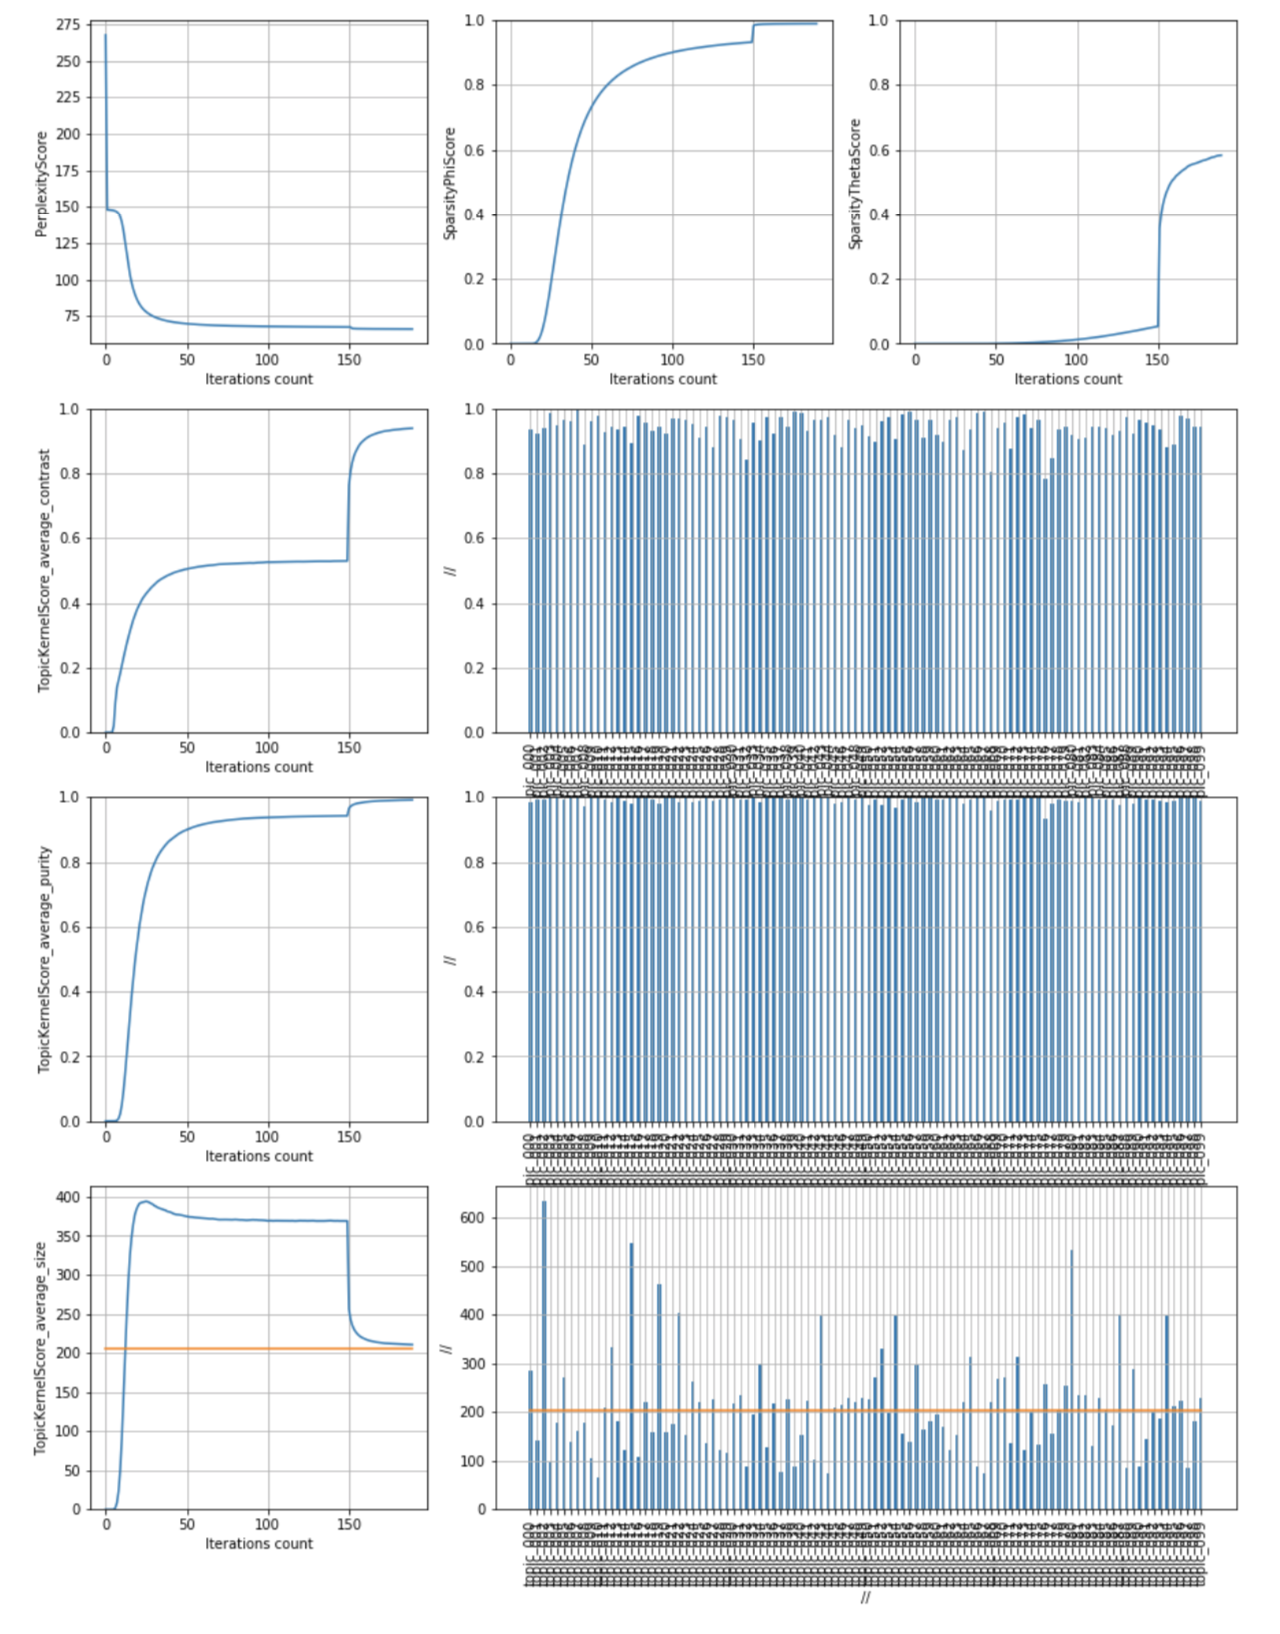
\includegraphics[scale=0.5]{vis_example.png}}
\caption{Пример визуализации результатов модели.}
\label{fig:vis_example}
\end{figure}

%
\section{Подготовка к запуску}

Для запуска решения необходимо установить:

\begin{itemize}
    \item \href{https://ipython.readthedocs.io/en/stable/}{ipython notebook} версии 7.5.0 и выше;
    \item библиотеку для тематического моделирования \href{https://bigartm.readthedocs.io/en/stable/installation/index.html}{BigARTM} для python3 версии 0.9.0 и выше;
    \item библиотеку для работы с html кодом \href{https://www.crummy.com/software/BeautifulSoup/}{BeautifulSoup} версии 4.7.1 и выше;
    \item библиотеку для лемматизации слов \href{https://pypi.org/project/pymystem3/}{pymystem3} для python версии 0.2.0 и выше.
\end{itemize}
